\documentclass[a4paper]{article}

%% Language and font encodings
\usepackage[english]{babel}
\usepackage[utf8x]{inputenc}
\usepackage[T1]{fontenc}

%% Sets page size and margins
\usepackage[a4paper,top=3cm,bottom=2cm,left=3cm,right=3cm,marginparwidth=1.75cm]{geometry}

%% Useful packages
\usepackage{amsmath}
\usepackage{amsfonts}
\usepackage{amssymb}
\usepackage{graphicx}
\usepackage[colorinlistoftodos]{todonotes}
\usepackage[colorlinks=true, allcolors=blue]{hyperref}

\title{\textbf{Teoría de Patrones: El modelo para música}}
\author{Jesús Joaquín Rojas, Rodolfo Ferro Pérez, María de Lourdes Oros Barrón.}
\date{28 de Noviembre del 2016.}

\begin{document}
\sffamily
\maketitle

\section{\sffamily Introducción}
Nuestro interés reside en construir un modelo para una señal dada $s(t)$ que viene de un instrumento musical. Naturalmente, para extraer más información de la señal, pensamos en llevarla a otra que dependa de las frecuencias de la misma, esto nos lleva a considerar la transfromada de Fourier de $s(t)$.\\
Por otro lado, análogo al capítulo anterior, para representar los patrones de la señal, necesitamos considerar en nuestro modelo variables aleatorias:
\begin{itemize}
\item El número $m$ de notas.
\item Los tiempos $t_{i}=k_{t}\Delta t$ en que las notas empiezan, $1 < k_{1} <k_{2}< \dots <k_{r}<N$.
\item Las frecuencias $\omega_{i}$ de las notas en Hertz, o bien los periodos $p_{i}=\frac{1}{\Delta t\cdot \omega_{i}} \in \mathbb{Z}$.
\end{itemize}
Se supondrá en adelante que la señal de sonido ha sido muestreada de manera discreta. Además, típicamente se considera que $\Delta t=\frac{1}{8000}$ de modo que si tomamos $5$ segundo de datos entonces $s_{k}=s(k\Delta t)$ con $1 \leq k \leq 40,000$. \\

\noindent Eventualmente definimos una función de densidad de probabilidad $p(\overrightarrow{s},m,\overrightarrow{t},\overrightarrow{p})$ sobre todas las variables para con ello reconstruir una nota de la señal observada $\overrightarrow{s}_{obs}$.\\

Tenemos entonces la tarea de resolver los siguientes problemas:
\begin{itemize}
\item Construir el modelo para la señal musical dadas observaciones $\overrightarrow{s}_{obs}$.
\item Encontrar un algorítmo que maximice $$p(m,\overrightarrow{t},\overrightarrow{p}|\overrightarrow{s}_{obs})=\frac{p(\overrightarrow{s}_{obs},m,\overrightarrow{t},\overrightarrow{p})}{\sum_{m',\overrightarrow{t'},\overrightarrow{p'}}p(\overrightarrow{s}_{obs},m',\overrightarrow{t'},\overrightarrow{p'})}.$$ respecto a las variables $m,\overrightarrow{t},\overrightarrow{p}.$
\item Optimizar los parámetros del modelo de manera que se ajuste a los datos tanto como sea posible.
\end{itemize}
En este trabajo se detallan los puntos anteriores de acuerdo al capítulo 2 de $\textit{Pattern Theory}$ de David Mumford. \\

\noindent Para el primer punto se rescata el análisis hecho en los capítulos $2.1-2.5$ para construir un modelo para notas, suponiendo en principio peridicidad de la onda. Una vez hecho lo anterior, partimos el espacio tiempo en intervalos $t_{i}$ correspondientes a comienzos de las notas. Luego se supone independencia de las variables en $[t_{i},t_{i+1})$ y se propone un modelo.\\

\section{\sffamily Distribuciones Gaussianas}
Sea $\overrightarrow{x} \in \mathbb{R}^{n}.$ Definimos la distribución Gaussiana en $\mathbb{R}^{n}$ por su función de densidad $$
p(\overrightarrow{x})=\frac{1}{Z}e^{-(\overrightarrow{x}-\overrightarrow{m})^{t} Q (\overrightarrow{x}-\overrightarrow{m})/2}
$$ donde $\overrightarrow{m}\in \mathbb{R}^{n}, Q$ es una matriz cuadrada de $nxn,$ definida positiva, simétrica y $Z$ es una constante tal que $\int p(\overrightarrow{x})d\overrightarrow{x}=1.$\\
La distribución Gaussiana tiene las siguientes propiedades:
\begin{itemize}
\item $Z=(2\pi)^{\frac{n}{2}} det(Q)^{-1}$.
\item $\int (\overrightarrow{x}-\overrightarrow{m})p(\overrightarrow{x})d\overrightarrow{x}=0$ donde $\overrightarrow{m}$ es la media.
\item Si $C_{ij}=\int (\overrightarrow{x_{i}}-\overrightarrow{m_{i}})(\overrightarrow{x_{j}}-\overrightarrow{m_{j}})p(\overrightarrow{x})d\overrightarrow{x}$ es la matriz de covarianza entonces $C=Q^{-1}$.
\end{itemize}
\textbf{Definición} Sea $p(x)$ es una función de densidad en $\mathbb{R}^{n}$, es decir, $dP=p(x_{1},\ddots,x_{n})dx_{1}\ddots dx_{n}$ es una medida de probabilidad. Entonces la entropia diferencial de $P$ se define como:
$$
H_{d}(P)=\int p(x)\log_{2}(\frac{1}{p(x)})dx.
$$\\
La distribución Gaussiana tiene la máxima entropía entre todas las distribuciones con media y varianza dadas.\\


\section{\sffamily La transformada de Fourier y algunas de sus propiedades.}

\subsection{\sffamily Transformada de Fourier y su inversa.}
Presentamos enseguida la transformada de Fourier en diferentes situaciones:\\
\begin{enumerate}
\item Dada una función $f\in L^{2}\mathbb{(R)},$ se define su transformada de Fourier como $$
\widehat{f}(\xi)=\int_{\mathbb{R}} \exp(-2\pi ix\xi)f(x)dx
$$ asi como su inversa
$$
f(x)=\int_{\mathbb{R}} \exp(2\pi i x\xi) \widehat{f}(\xi)d\xi.
$$
$x$ representa el tiempo y $\xi$ la frecuencia de $f.$
\\
\item Si $\{f_{n}\}_{n} \in l^{2}$ es una sucesión de funciones entonces la transformada de Fourier de tal sucesión es la función de periodo uno
$$
\widehat{f}(\xi)=\sum_{n=-\infty}^{\infty} \exp(-2i\pi n\xi)f_{n}
$$ con $f_{n}=\int\limits_{0}^{1}\exp(2i\pi n\xi) \widehat{f}(\xi)d\xi.$
\\
\item Si $f$ es una función de $x$ de periodo $1$, entonces los coeficientes de Fourier $f_{n}$ de $f$ para $n\in \mathbb{N}$ y la formula de inversión inversa son:
$$
\widehat{f_{n}}=\int_{0}^{1}f(x)\exp(-2\pi inx)dx
$$ y $$
f(x)=\sum_{n=-\infty}^{\infty} \widehat{f_{n}}\exp(2i\pi nx)
$$ respectivamente.
\\
\item Si $(f_{0},f_{1},...,f_{N})$ es una sucesión de funciones entonces su transformada discreta de Fourier así como su inversa son respectivamente:
$$
\widehat{f_{m}}=\frac{1}{\sqrt[]{N}}\sum_{n=0}^{N-1}\exp\left(-2\pi i\frac{nm}{N}\right)f_{n};
$$ $$
f_{m}=\frac{1}{\sqrt[]{N}}\sum_{n=0}^{N-1}\exp\left(2\pi i\frac{nm}{N}\right)\widehat{f_{n}}.
$$
\end{enumerate}

\subsection{\sffamily Algunas propiedades importantes.}
\begin{enumerate}
\item Isometría$\left \| f \right \|_{2}=\left \| \widehat{f} \right \|_{2}.$
\item Convolución $\widehat{fg}=\widehat{f} \ast \widehat{g}$ y $\widehat{f\ast g}=\widehat{f} \widehat{g}.$
\item Traslación $\widehat{f(x-a)}=\exp(-2\pi ia\xi)\widehat{f}$ y $\widehat{f}(\xi-a)=\widehat{\exp(-2\pi ia\xi)}f.$ 
\item Producto por escalar $\widehat{f(ax)}=\frac{1}{a}\widehat{f}(\frac{x}{a}).$
\item Cauchy: $\widehat{\exp(-2\pi |x|)}=\frac{1}{\pi(1+x^{2})}.$
\item Propiedad Gaussiana:
$$
\widehat{e^{\frac{-x^{2}}{2\sigma ^{2}}}}=\sqrt[]{2\pi}\sigma e^{-2\pi^{2}\sigma^{2}\xi^{2}}.
$$
\end{enumerate}

\section{\sffamily Modelos Gaussianos para notas musicales}
\subsection{\sffamily Modelos Gaussianos para señales cíclicas finitas.}
Sea $\overrightarrow{s}=(s_{0},\dots,x_{N-1})$ una señal periódica y $\overrightarrow{f}^{k}=\frac{1}{\sqrt[]{N}}(1,e^{2i\pi\frac{k}{N}},\dots,e^{2i\pi\frac{k(N-1)}{N}})$ para $0 \leq k \leq N-1$ la base de Fourier.\\
Podemos entonces expresar la señal dada en esta base, usando la transformada inversa, como: 
$$
\overrightarrow{s}=\sum_{l=0}^{N-1}\overrightarrow{s_{l}}\overrightarrow{f}^{l}
$$\\
\textbf{Teorema} Una distribución Gaussiana $p_{Q}$ es estacionaria si y solo si $\overrightarrow{m}$ es constante y $Q$ es una matriz bandada hermitiana ($Q_{ij}$ depende solo de $j mod N$ y $a_{j}=\overline{a_{N-j}}$).

\subsection{\sffamily El caso de una nota musical.}
Se construye un modelo Gaussiano de una nota.\\

\noindent Si $\omega$ es la frecuencia fundamental de la nota, entoces $p=1/\omega$ es su periodo. Si $s(t)$ es la señal entonces $s(t+p)\approx s(t).$ Consideramos entonces que la señal es periódica y expandimos en series de Fourier con frecuencias $n/p$ donde $n$ es el tamaño del muestreo.\\

\noindent Formalizamos la priopiedad $s(t+p)\approx s(t)$ suponiendo que el valor esperado $\int (s(t+p)-s(t))^{2} dt$ es muy pequeño y a la vez acotamos la potencia de la señal $\int s(t)^{2} dt.$\\

\noindent Tomemos un muestreo aleatorio de la señal $s$ y supongamos que $s_{N+k}=s_{k}$ para algun $N$ y sea $q=N/p$ el número de cíclos, para algún natural p.\\

\noindent La función de densidad del modelo más simple posible de una distribución Gaussiana para $s$ es: 
$$
p_{a,b}(s)=\frac{1}{Z}e^{-a\sum_{k=0}^{N-1}(s(k)-s(k+p))^{2}/2-b\sum_{k=0}^{N-1}s(k)^{2}/2}=\frac{1}{Z}e^{-\overrightarrow{s}^{t}Q\overrightarrow{s}/2}
$$ donde $a >> b > 0, Q_{ii}=2a+b, Q_{i,i+p}=-a.$ $p_{a,b}$ es una distribución estacionaria.\\
En las bases de Fourier 
$$
p_{a,b}(s)=\frac{1}{Z}\prod_{l}e^{-(b+4asin(\frac{\pi pl}{N})^{2}|\hat{s}(l)|^{2}/2}
$$
\subsection{\sffamily Discontinuidades en señales de dimensión uno}
Las notas se descomponen en compaces, tonos, melodías etc. Naturalmente las señales tiene estructuras jerárquicas separadas por varios tipos de discontinuidades a las que llamaremos patrones geométricos. Tales discontinuidades son consideradas en este contexto como saltos muy grandes en los datos, esto se estudia vía kurtosis.  

%%%%%%%%%%%%%%%%%%%%%%%%%
\section{\sffamily El modelo para música}
Sea $s(t)$ una señal, y como antes, supongamos que la hemos discretizado. Supongamos ahora que $m$ el número de notas, $\overrightarrow{t}$ el vector de tiempos en que inician las mismas, $\overrightarrow{p}$ el vector de periodos están dados. De la ley de probabilidad condicional $$
p(\overrightarrow{s},m,\overrightarrow{t},\overrightarrow{p})=p(\overrightarrow{s}|m,\overrightarrow{t},\overrightarrow{p})p(m,\overrightarrow{t},\overrightarrow{p}).
$$
De esta manera, la distribución de probabilidad $p(\overrightarrow{s},m,\overrightarrow{t},\overrightarrow{p})$ se puede descomponer como sigue:
$$
p(\overrightarrow{s},m,\overrightarrow{t},\overrightarrow{p})=\prod_{l=1}^{m} p((\overrightarrow{s}|I_{l})|p_{l},t_{l},t_{l+1})p(\overrightarrow{p},\overrightarrow{t},m)
$$ donde $I_{l}=\{t| t_{l}\leq t < t_{l+1}\}$ y $t_{l}$ con $l \in \{1,\dots, m\}$ son los intervalos de tiempo en que inician las notas. En la expresión anterior se supone que en cada periodo $[t_{l},t_{l+1})$ las notas son independientes e identicamente distribuidas con distribución Gaussiana.\\

\noindent Se construyó un modelo Gaussiano para las notas en las secciones pasadas $(4.2)$ $$p((\overrightarrow{s}|_{I_{l}})|p_{l},t_{l},t_{l+1})
=\frac{1}{Z}exp(-a\sum_{n=t_{l}}^{t_{l+1}-p_{l}-1}(s_{n+p_{l}}-s_{n})^{2}/2-b\sum_{n=t_{l}}^{t_{l+1}-1}s_{n}^{2}/2)
$$ con $a>>b.$
Un modelo geométrico muy simple para esto se obtiene tomando $\overrightarrow{t}$ con distribución Poisson y cada $p_{l}$ independiente de los otros periodos.\\

Vamos a describir al algoritmo de programaci\'on din\'amica aplicado en este contexto.
Recordemos que queremos maximizar el valor $p(\vec{s},m,\vec{t},\vec{p})$ en funci\'on
de las variables $m,\vec{t},\vec{p}$ y fijo $\vec{s}=\vec{s}_0$. Usando el modelo gausiano
obtuvimos una expresi\'on para $p$.\\
Definamos la funci\'on $E(m,\vec{t},\vec{p})=-\log(p(\vec{s}_0,m,\vec{t},\vec{p}))$, la cual tiene
la siguiete forma $\sum_{k=1}^{m}f(t_k,t_{k+1},p_k)$. Consideremos todos los posibles valores
de p en $[0,t]$ suponiendo que una \'ultima nota termina en el tiempo $t$. Dicha nota empieza al tiempo
$t'+1<t$ y tiene un periodo $p$. Entonces la funci\'on $E$ tiene la siguiente forma
\begin{equation}
 E=E_1\Big(\vec{s}_0|_{[0,t']} \text{notas antes de }t'\Big) + E_2\Big(\vec{s}_0|_{[t'+1,t]}p\Big)
\end{equation}
La funci\'on $E_1$ toma en cuenta los primero $k-1$ sumandos de $E$. Definamos
\begin{equation}
 e(t'):=\min_{}E_1\Big(\vec{s}_0|_{[0,t']} \text{notas antes de }t'\Big)
\end{equation}
donde el m\'inimo se toma sobre todas las ternas factibles $(m,\vec{t},\vec{p})$ tales que 
$t_{k-1}=t'+1$. Supongamos que conocemos todos los valores de $e$  para $t'<t$. Entonces
seg\'un el algoritmo de programaci\'on din\'amica, el valor m\'inimo para $E$ es
\begin{equation}
 e(t)=\min_{t'<t}\big[ e(t')+E_2\Big(\vec{s}_0|_{[t'+1,t]}p\Big) \big],
\end{equation}
suponiendo que la \'ultima nota termian en el tiempo $t$. Esto nos da una soluci\'on para 
el m\'aximo valor de $p$.

%%%%%%%%%%%%%%%%%%%%%%%%%%%%
\section{\sffamily Sintetizando música}

\noindent Esta sección incluye un \textit{Jupyter Notebook} con el código de implementación sobre lo expuesto. El cuaderno \href{https://github.com/RodolfoFerro/SynthesizingMusic/raw/master/Synthesizing\%20music.ipynb}{\texttt{Synthesizing music.ipynb}} utiliza los widgets que por default \texttt{IPython} ya tiene incluidos, por lo que no es necesaria la instalación de alguna librería extra. El cuaderno sigue los subtemas en el orden expuesto y se encuentran comentados, de manera tal que sólo es requerido correr las celdas sin problema alguno.\\

\subsection{\sffamily ¿Qué es un sintetizador?}
\noindent De manera sencilla, un sintetizador es un instrumento musical electrónico que genera señales eléctricas convertidas a sonidos a través de bocinas o auriculares. Los sintetizadores pueden imitar sonidos de instrumentos o generar nuevos timbres. A continuación, construimos un sintetizador utilizando Python, basándonos en el problema 3 "Synthesizing music" del libro.\\

\subsection{\sffamily ¿Cómo sintetizar música utilizando Python?}
\noindent De acuerdo a Mumford, la forma más sencilla de sintetizar muestras aleatorias de un proceso Gaussiano estacionario es escogiendo coeficientes de Fourier de una distribución Gaussiana con media cero y varianza cualquiera que se desee y luego tomando la transformada de Fourier.

\subsubsection{\sffamily Sintetizando ruido de color con \textit{power law power spectrum}}
\noindent En otras palabras, tómese la parte real e imaginaria de los coefficientes de Fourier $\hat{s}_k$, $0 \leq k < N$ como variables aleatorias con media 0 y desviación estándar $1/ \min(k, N − k)^\lambda$, pero con $\hat{s}_0 = 0$, $\hat{s}_{N −k} = \hat{s}_k $. Nótese que las frecuencias más bajas provienen de los coeficientes de Fourier con índice cerca de cero o cerca de $N$. ¿Una primera aproximación? Tómese el tamaño del vector, $N$, como 1024. Hágase esto para $\lambda$ = 0, 0.5, 1 y 2 y grafíquense los resultados.
\begin{center}
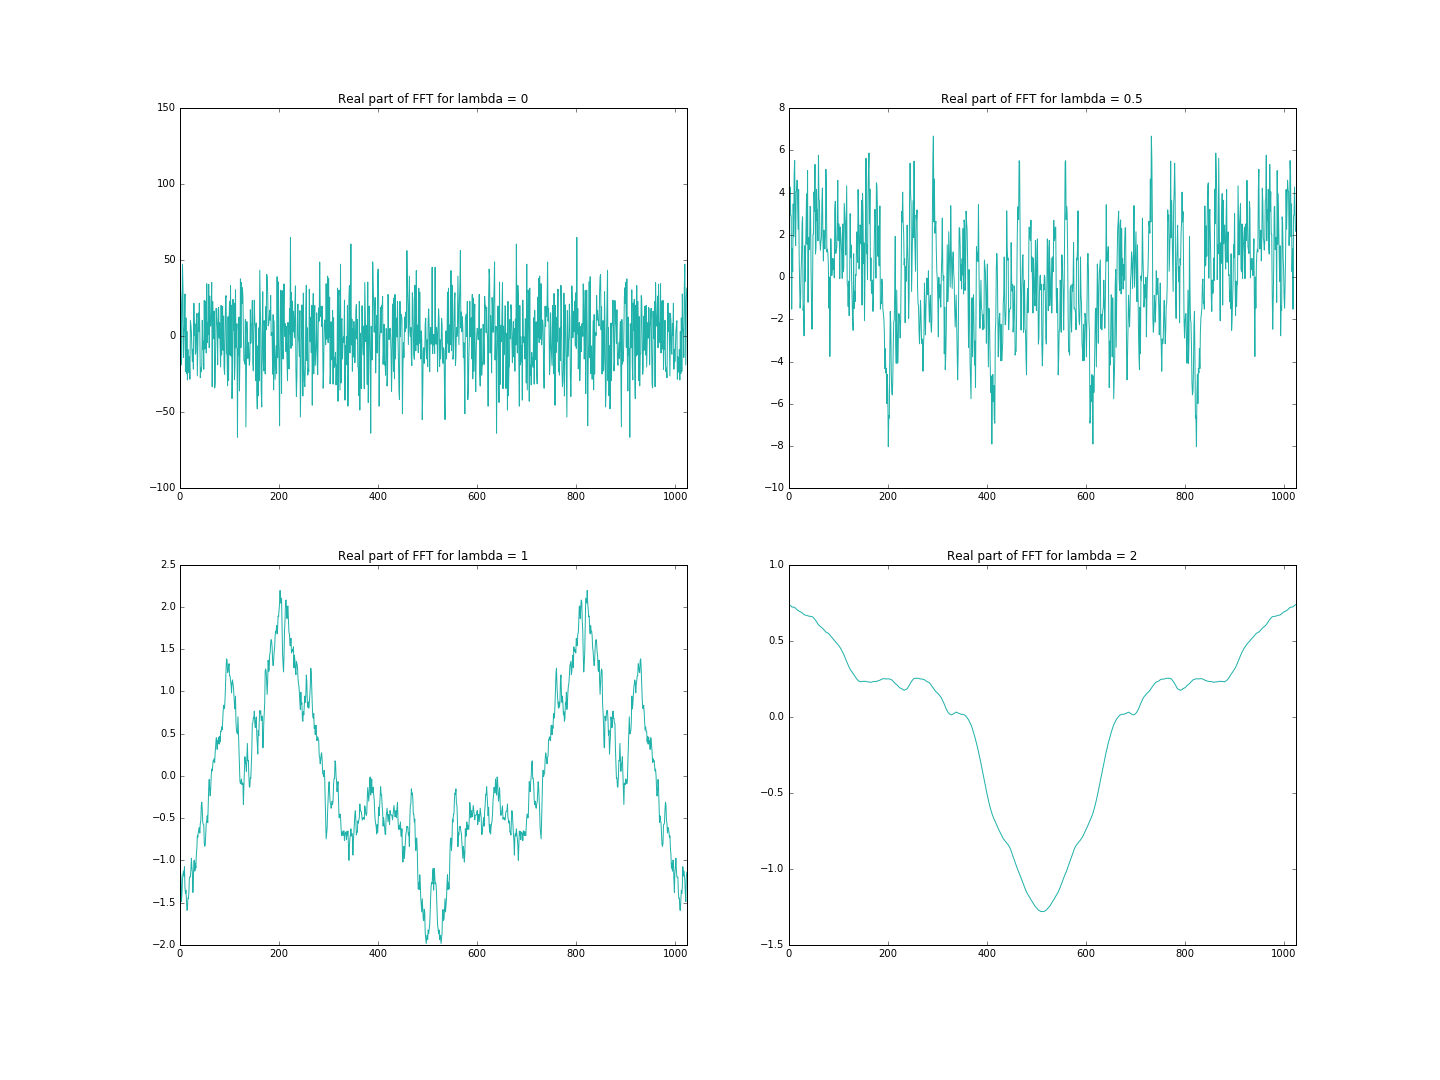
\includegraphics[width=0.49\textwidth]{real_noise}
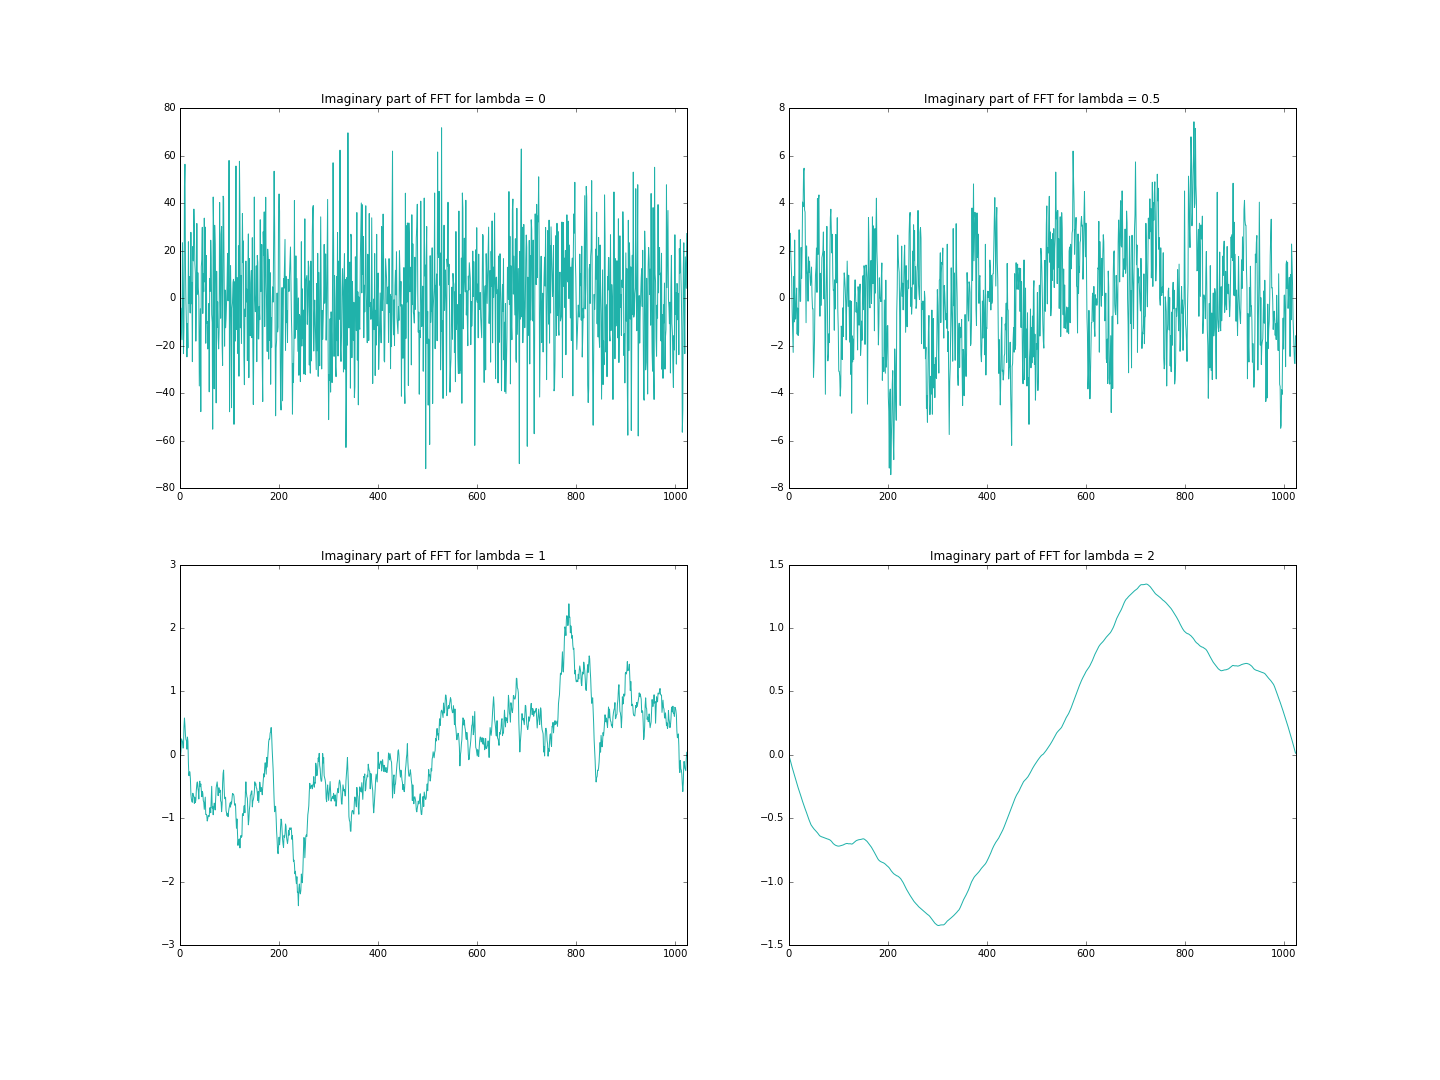
\includegraphics[width=0.49\textwidth]{imag_noise}\\
\textsc{Figura 1. a) Parte real para diferentes $\lambda$ \\b) Parte imaginaria para diferentes $\lambda$.}\\
\end{center}

\noindent \\De las gráficas anteriores puede observarse que existe simetría respecto a los ejes, de manera diferente para la parte real y la imaginaria; y ya pueden ser reproducidas utilizando la función \texttt{Audio()} que se encuentra en el módulo \texttt{Audio} de \texttt{IPython.display}. Esto cargará un widget del \textit{Jupyter Notebook} que reproducirá sonido. Podrá observarse que la duración del audio es corta, por lo que la recomendación es definir un factor de longitud para tomar una muestra aún mayor que cree un audio de mayor duración. En la reproducción puede percibirse también que para los diferentes lambdas se escucha "suavidad" en el sonido, lo que se interpreta como el color del ruido generado. Hasta este punto, ya hemos generado ruido que se escucha como la estática de la televisión, con "suavidad" variada.\\

\noindent En este momento, hay que hacer notar algo muy importante en relación a los resultados obtenidos hasta ahora: el ruido es sonido con una forma de onda irregular, mientras que una nota musical es sonido con una forma de onda regular. En la \textsc{Figura 2} se ilustra este concepto, mostrando incluso la onda que genera el sonido de un piano y de un violín.
\begin{center}
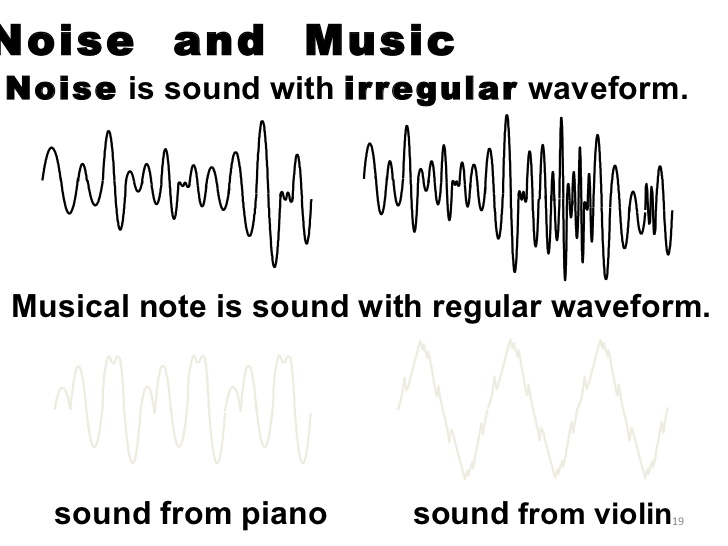
\includegraphics[width=0.5\textwidth]{soundwaves}\\
\textsc{Figura 2. Diferencia entre ruido y nota musical.}\\
\end{center}

\subsubsection{\sffamily Sintetizando notas musicales únicas y aleatorias de música}
\noindent Se sintetizan notas musicales únicas y aleatorias de música tomando la distribución Gaussiana. Aquí, $s(k)$ se asume que "envuelve" por encima a $N$ (i.e., $s_{N+k} = s_k$). Tómese $N = 8192$, $p = 32$, y $q = N / p$ determinará el número de ciclos que hay la señal de tamaño $N$. Dicho en otras palabras, se genera una muestra de tamaño $p$ y se concatena $q$ veces para formar el sonido. Esto hace sentido si se tiene en mente lo antes mencionado sobre el ruido y una nota musical, pues se está generando la nota musical a partir de ruiso, concatenando ruido para tener una forma de onda regular. El resultado de esto se percibe como un sonido electronico parecido a un timbre.

\subsubsection{\sffamily Revisando el \textit{power spectrum} (espectro potencia)}
\noindent Teniendo una señal (nota musical en este caso), puede tomarse la \textit{FFT} y obtener una nueva señal simétrica (como se ha visto en las primeras partes de esta sección), tomando el valor absoluto y la mitad (pues es simétrica) se obtiene el \textit{power spectrum}, lo que se interpreta como la gráfica espectral con la nota funcamental y los armónicos de la señal.

\begin{center}
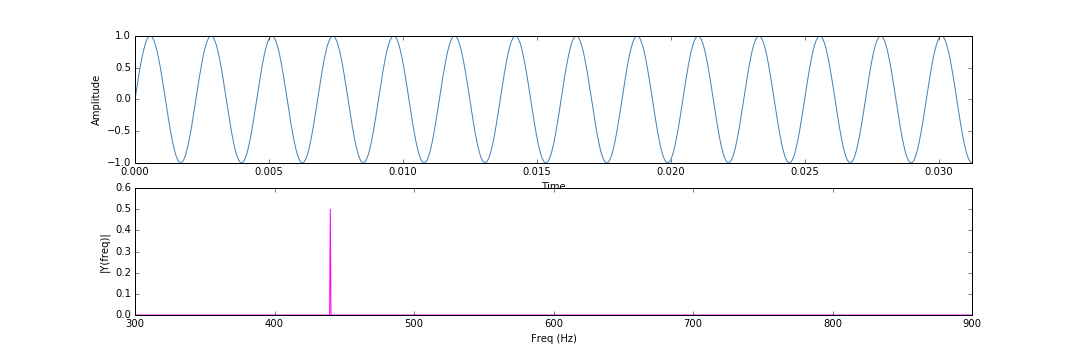
\includegraphics[width=0.9\textwidth]{spec}\\
\textsc{Figura 3. La señal es una onda sinusoidal (un sólo tono) con frecuencia de 440 Hertz, por lo que el espectro sólo muestra un pico en 440.}\\
\end{center}

\subsubsection{\sffamily Jugando un poco...}

\noindent En la sección "Let's play a bit!" del cuadernillo, se muestra la misma imagen que en la \textsc{Figura 4}, con ejemplos de ondas de instrumentos, las cuales pueden ser generadas a partir de ruido como se mostró, variando solamente la frecuencia, amplitud, etc. En esta misma parte se ilustra la manera de realizar concatenaciones usando \texttt{numpy.concatenate()} entre las señales generadas y puede escucharse el sonido generado en ese ejemplo. Dicha sección es libre de edición para el lector/usuario del cuaderno, con la propuesta de generar ruido y utilizar partes del ruido generado para aproximar el sonido de algún instrumento.\\

\begin{center}
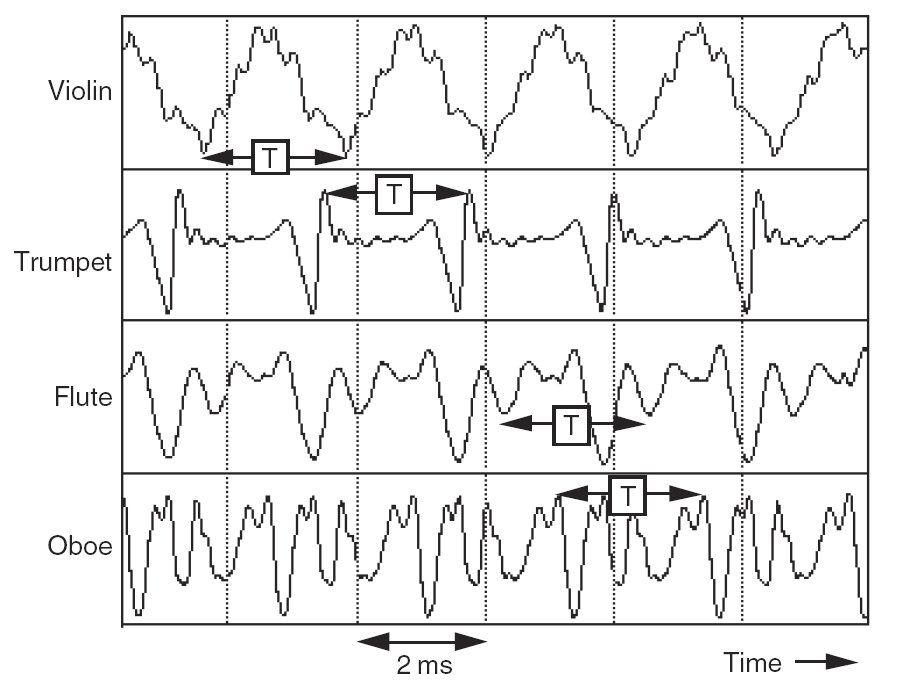
\includegraphics[width=0.5\textwidth]{examples}\\
\textsc{Figura 4. Ejemplos de ondas de sonido generadas por algunos instrumentos.}
\end{center}

\subsubsection{\sffamily Videos recomendados}
\begin{enumerate}
\item \href{http://www.youtube.com/watch?v=PU8M0eIqgy4}{\textit{Simple additive synth}}. Implementación con interfaz gráfica de un sintetizador de sonido utilizando Python. Extra:
\begin{itemize}
\item Revisar el \href{https://github.com/Penguinum/python-synth}{github} del autor.
\end{itemize}
\item \href{http://www.youtube.com/watch?v=0ALKGR0I5MA}{Basic Sound Processing in Python | SciPy 2015 | Allen Downey.} Presentación de \textit{Allen Downey}, autor del libro "Think DSP: Digital Signal Processing in Python", en \textit{SciPy 2015}. En ella explica su trabajo realizado en relación al pricesamiento de sonido utilizando Python. Extra:
\begin{itemize}
\item Revisar el \href{http://greenteapress.com/thinkdsp/html/index.html}{sitio web} del libro del autor.
\item Revisar la versión en \href{http://greenteapress.com/thinkdsp/thinkdsp.pdf}{PDF} del mismo.
\item Revisar el \href{https://github.com/AllenDowney/ThinkDSP}{github} del autor.
\end{itemize}
\end{enumerate}

%%%%%%%%%%%%Bibliografía
\begin{thebibliography}{96}
\expandafter\ifx\csname
natexlab\endcsname\relax\def\natexlab#1{#1}\fi

\bibitem{Pattern Theory.}
Pattern Theory. David Mumford. \textit{Ch2}

\bibitem{Thin DSP}
Think DSP: http://greenteapress.com/thinkdsp/thinkdsp.pdf

\bibitem{Jupyter Notebook}
Github: https://github.com/RodolfoFerro/SynthesizingMusic

\end{thebibliography}
\end{document}

\end{document}
